%%%%%%%%%%%%%%%%%%%%%%%%%%%%%%%%%%%%%%%%%
% Journal Article
% LaTeX Template
% Version 1.3 (9/9/13)
%
% This template has been downloaded from:
% http://www.LaTeXTemplates.com
%
% Original author:
% Frits Wenneker (http://www.howtotex.com)
%
% License:
% CC BY-NC-SA 3.0 (http://creativecommons.org/licenses/by-nc-sa/3.0/)
%
%%%%%%%%%%%%%%%%%%%%%%%%%%%%%%%%%%%%%%%%%

%----------------------------------------------------------------------------------------
%	PACKAGES AND OTHER DOCUMENT CONFIGURATIONS
%----------------------------------------------------------------------------------------

\documentclass[twoside]{article}

\usepackage{lipsum} % Package to generate dummy text throughout this template
\usepackage{graphicx}

\usepackage[sc]{mathpazo} % Use the Palatino font
\usepackage[T1]{fontenc} % Use 8-bit encoding that has 256 glyphs
\linespread{1.05} % Line spacing - Palatino needs more space between lines
\usepackage{microtype} % Slightly tweak font spacing for aesthetics

\usepackage[hmarginratio=1:1,left=20mm, top=32mm,columnsep=20pt]{geometry} % Document margins
\usepackage{multicol} % Used for the two-column layout of the document
\usepackage[hang, small,labelfont=bf,up,textfont=it,up]{caption} % Custom captions under/above floats in tables or figures
\usepackage{booktabs} % Horizontal rules in tables
\usepackage{float} % Required for tables and figures in the multi-column environment - they need to be placed in specific locations with the [H] (e.g. \begin{table}[H])
\usepackage{hyperref} % For hyperlinks in the PDF

\usepackage{lettrine} % The lettrine is the first enlarged letter at the beginning of the text
\usepackage{paralist} % Used for the compactitem environment which makes bullet points with less space between them

\usepackage{abstract} % Allows abstract customization
\renewcommand{\abstractnamefont}{\normalfont\bfseries} % Set the "Abstract" text to bold
\renewcommand{\abstracttextfont}{\normalfont\small\itshape} % Set the abstract itself to small italic text

\usepackage{titlesec} % Allows customization of titles
\renewcommand\thesection{\Roman{section}} % Roman numerals for the sections
\renewcommand\thesubsection{\Roman{subsection}} % Roman numerals for subsections
\titleformat{\section}[block]{\large\scshape\centering}{\thesection.}{1em}{} % Change the look of the section titles
\titleformat{\subsection}[block]{\large}{\thesubsection.}{1em}{} % Change the look of the section titles

\usepackage{fancyhdr} % Headers and footers
\pagestyle{fancy} % All pages have headers and footers
\fancyhead{} % Blank out the default header
\fancyfoot{} % Blank out the default footer
%\fancyhead[C]{Some title $\bullet$ April 2015 $\bullet$ Vol. XXI, No. 1} % Custom header text
\fancyfoot[RO,LE]{\thepage} % Custom footer text

\renewcommand{\thesubsection}{\Alph{subsection}}

%----------------------------------------------------------------------------------------
%	TITLE SECTION
%----------------------------------------------------------------------------------------

\title{\vspace{-15mm}\fontsize{24pt}{10pt}\selectfont\textbf{Device Agnostic W-LAN Fingerprint Positioning for Consumer Applications}} % Article title

\author{
\large
\textsc{Brett Fischler, Daniel Griffin, Tyler Lubeck, and Hunter Wapman}\\
%\thanks{A thank you or further information}\\[2mm] % Your name
\normalsize Tufts University\\ % Your institution
\normalsize \href{mailto:teamsirius@gmail.com}{teamsirius@gmail.com} % Your email address
\vspace{-5mm}
}
\date{}

%----------------------------------------------------------------------------------------

\begin{document}

\maketitle % Insert title

\thispagestyle{fancy} % All pages have headers and footers

%----------------------------------------------------------------------------------------
%	ABSTRACT
%----------------------------------------------------------------------------------------

\begin{abstract}

\noindent 
The goal of this work is to demonstrate the viability of a fingerprinting-based indoor positioning application in an environment facing constraints similar to a commercial setting. In our work, we propose solutions to commercial implementation challenges such as heterogeny of wireless devices, limited site-access, access point position blindness, positioning latency, application scalability, and site-survey time. We implement several methods to improve the performance of our positioning application, including fingerprint-map modification and distance function improvements.

\end{abstract}

%----------------------------------------------------------------------------------------
%	ARTICLE CONTENTS
%----------------------------------------------------------------------------------------

\begin{multicols}{2} % Two-column layout throughout the main article text

\section{Introduction}
\lettrine[nindent=0em,lines=3]{L}ocation context is becoming increasingly important in consumer applications. Although methods for outdoor positioning such as GPS and radio tower triangulation are widespread, several factors such as line of sight make indoor positioning significantly more difficult and decrease accuracy. Finding an indoor location of a Wireless Device (WD) can more accurately be addressed with signal-based positioning utilizing WiFi information including Received Signal Strength (RSS), Angle of Arrival (AOA), and Time of Arrival (TOA).\\
\indent In general, TOA and AOA measurements are used with trilateration and triangulation, respectively, which both require prior knowledge about the position of access points in the site. Furthermore, both TOA and AOA measurements are susceptible to the multipath effect, which can result in inadequate accuracy. \\
\indent RSS measurements can be effectively used for wireless indoor positioning by utilizing a fingerprint (FP) map and a classifying algorithm. Each FP has a unique position on a map-image, as well as a set of MAC addresses and corresponding RSS values. This FP map can be created in two ways: manual site-survey or site-simulation. Site-simulation techniques, like triangulation and trilateration methods, require prior information about AP positions, something we were keen to avoid. Therefore, we opted for manual site-survey, as the approach imposes the fewest constraints upon the site. Furthermore, by manually surveying the site, there are no additional calculations to account for the multipath effect, as its effect is captured in the recording.\\
\indent Additionally, non-signal-based data may be incorporated into the positioning application, such as the WD?s inertia or prior knowledge of the site. These techniques have been shown to significantly improve positioning accuracy. We implement two novel site-blind techniques for improving our position finder: neighbor-weighting points in the FP database, and initial-floor detection using the Jaccard metric.\\
\indent This work is organized in the following way: we first discuss the architecture of our positioning application, describing the methods we used to create the FP database and the characteristics of our positioning algorithm. We then present a performance evaluation of our application. In our final section, we discuss possible extensions to our work, as well as conclusions. 

%------------------------------------------------

\section{Indoor Positioning System}

\indent This positioning system is intended to be used by a human operator to determine the position of some other wireless device in a building. The application should provide the same services as GPS with precision and accuracy suitable to an indoor environment. Therefore, a basic positioning application must provide at least room-level accuracy and real-time feedback.\\
\indent Though a number of applications satisfying these criteria have been proposed, indoor-positioning applications have yet to see widespread implementation. The primary goal of this work is therefore to demonstrate the viability of an indoor positioning application in an environment facing constraints similar to a commercial setting. \\
\indent In addition to the basic requirements of a positioning system outlined above, an indoor-positioning system for use in commercial settings must meet several criteria: it should be useable on variety of devices; it must be able to serve multiple users simultaneously; the application should not be too costly to implement; the application should make as few assumptions as possible about the building; and lastly, the application should be adaptable to different runtime/accuracy demands.\\
\indent In our work, we propose solutions to commercial implementation challenges such as heterogeneity of wireless devices, limited site-access, access point position blindness, positioning latency, application scalability, and site-survey time. We implement several methods to improve the performance of our positioning application, including fingerprint-map modification and distance function improvements. \\
\indent Our application is based on the client server model, which uses a single central server to serve a large number of clients [8]. The server manages the map database and uses HTTP to respond with our position estimate upon receiving a request containing a fingerprint (FP). This approach is hardware-agnostic, an important capability for commercial application, and also allows simultaneous FP recording on multiple WDs, significantly speeding up the site-survey process. \\
\indent Our application could be modified for higher accuracy (at the cost of mapping time) or lower mapping time (at the cost of accuracy). We provide quantitative analysis of how different decisions affected the performance of our positioning application, balancing positioning accuracy against mapping time and effort. 

%------------------------------------------------

\section{Mapping}

\subsection{Environment}

\indent We mapped two floors of Halligan Hall, the Computer Science building at Tufts University. The floor plans were available to us, but the locations of the wireless access points were not disclosed. Furthermore, there are several areas in the building which we did not have access to, like restrooms and offices. These are similar to the constraints one would expect to find in a commercial environment, where access is restricted, network hardware cannot be modified, and the available site information is minimal. A contour map was generated in order to examine the number of unique MAC addresses visible at each accessible location. Unsurveyed areas were assumed to have 0 visible MAC addresses.

\includegraphics[width=\linewidth]{contour}
\begin{center}
Figure 1
\end{center}

\subsection{Fingerprint Logging Methodology}

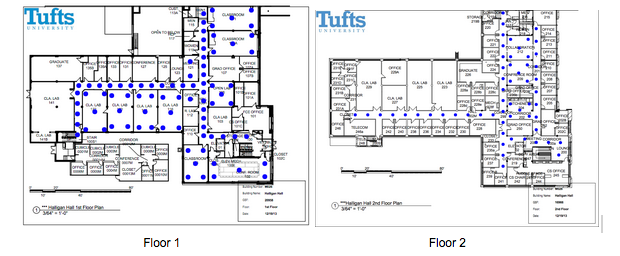
\includegraphics[width=\linewidth]{locations}
\begin{center}
Figure 2 - Mapped Positions in Halligan
\end{center}
          
     
\indent To build the FP database, the average of thirty RSS scans is logged for each position, indicated in Figure 2. The positions in Figure 2 were determined manually through an examination of the floor plans and knowledge of the facilities accessibility. Each recording was stored as four values, a MAC address string, a float RSS value, a float standard deviation, and an association with a location on a map. The recordings were taken at positions found using human estimation based on visual examination of a single circular mark on the floor map for each location.\\
\indent In deciding on the number of scans, we considered three factors: time, RSS precision, and MAC address coverage. We tested a sample of scan values between one and one hundred using a single WD. The average Euclidean distance between each of the scans was under 1 -db when using E (discussed in section II.ii.A). Given the similarity of RSS values, we decided to focus on the remaining two factors, time and MAC coverage. 

\vspace{5mm}
\resizebox{\columnwidth}{!}{%
\begin{tabular}{cccccc}
MAC Coverage(\%) & 2 Scans & 10 Scans & \textbf{30 Scans} & 60 Scans & 100 Scans \\
Trial 1                & 85.3    & 91.2     & \textbf{96.1}     & 100      & 100       \\
Trial 2                & 88.7    & 90.3     & \textbf{96.8}     & 100      & 100       \\
Trial 3                & 74.4    & 79.5     & \textbf{89.2}     & 97.6     & 100       \\
Trial 4                & 59.6    & 84.3     & \textbf{95.5}     & 97.8     & 100       \\
Average                & 77.0    & 86.3     & \textbf{94.4}     & 98.9     & 100          
\end{tabular}
}
\begin{center}
Table 1
\end{center}
	
\indent Increasing the number of scans improves results, but involves a time-tradeoff, as scanning is the most time consuming part of site-survey. In regards to runtime, different WDs had dramatically different scan times, ranging from ? of a second to 7.5X that value. The table below lists the approximate floor recording time each scan-number would require, assuming the worst-case scan time.\\
	
\vspace{5mm}
\resizebox{\columnwidth}{!}{%
\begin{tabular}{cccccc}
Scans (1.5s/scan) & 2 & 10 & \textbf{30} & 60 & 100 \\
Time(Hours )               & 0.24   & 1.2     & \textbf{3.5}     & 7.0      & 12
\end{tabular}
}
\begin{center}
Table 2
\end{center}
	
\indent As one of our goals was to provide device-agnostic indoor positioning, we chose a number of scans for site-survey which balanced sufficient RSS precision and against worst-case device runtime. Given the MAC coverage similarity between 30 scans and 100 scans and the runtime implications of each, we opted for 30 scans. \\
\indent When recording the FP database, four devices were utilized: the HTC One m7 (Wi-Fi: IEEE 802.11 a/ac/b/g/n), LG Nexus 4  (Wi-Fi: IEEE 802.11 b/g/n), Samsung Galaxy S3 (Wi-Fi: Wi-Fi 802.11 a/b/g/n), and the Samsung Galaxy Nexus(Wi-Fi: IEEE 802.11 a/b/g/n). The average distance between each phone?s recording of the same physical location was 6.3 -dB. This value is notably high compared to an average distance of 1.7 -dB between four surveys made using the same phone. Though detrimental to our position finder?s accuracy, the decision to map with multiple devices is a reflection of our desire to build a device-agnostic system. Further, supporting all device types significantly sped up the mapping process, as parallel mapping was possible.\\
\indent A final consideration was the direction of the recording device. Direction has been shown to have an effect on measurements [1]. We found an average distance of 4.0 -dB between four surveys made with the same WD in the same position. We decided to map facing a single direction as this reduced mapping-time by a factor of four. Our implementation does, however, support mapping with direction for applications requiring higher accuracy.\\
\indent The set of FPs collected during mapping is used as data for our positioning algorithm. Upon receiving a positioning request containing FP A, the algorithm compares A with each FP in the mapped set, using the FPs most similar to A to estimate A?s position on the map.

%------------------------------------------------

\section{Algorithm}

\subsection{Weighted K-Nearest Neighbor}

\indent Many classifiers are suitable for determining the location of an unknown point given an RSS Fingerprint map [2][3]. In our implementation we use the deterministic Weighted K-Nearest Neighbor (WKNN) method to perform position estimation.\\
\indent Consider a set S of FPs  where N=[$n_1$, $n_2$, ..., $n_K$] is the set of K FPs from S nearest to some other point $\rho$ by distance function $\sigma$, which quantifies distance as a function of RSS. The estimated location $\rho$ is calculated as:
\begin{equation}
\label{wknn}
\hat{\rho} = \sum\limits_{i=1}^{K}\frac{\omega_i}{\omega_{total}}\rho'_i
\end{equation}
\indent where $\omega_i$ is the weight of $n_i$, $\rho'_i$ is the position corresponding to $n_i$, and $\omega_{total}$ is the sum of the weights of all FPs in N. The K-Nearest Neighbor (KNN) method uses equal weights for all fingerprints in N[5]. For our implementation, the weight $\omega_i$ of FP $n_i$ is calculated as the inverse of $\sigma(n_i, \rho)$, the signal distance between $n_i$ and $\rho$ using distance function $\sigma$. The specific distance functions used in our implementation are discussed in the next section. We use WKNN because it has been shown to have a higher accuracy than merely the Nearest Neighbor (NN) method, K = 1, yielding best results with K values of 3 or 4 [5]. 
	
\subsection{Distance Functions}

\indent WKNN is a very flexible classifier, and can incorporate a variety of distance functions. In this section, we discuss the four distance functions we used to quantify difference between two RSS measurements: Euclidean distance ($\sigma_E$), penalty-weighted Euclidean distance ($\sigma_{E'}$), inverse Jaccard coefficient ($\sigma_{J^{-1}}$), and a linear combination of $\sigma_{E'}$ and $\sigma_{J^{-1}}$ ($\sigma_{E' + J^{-1}}$). For consistency in our definitions, we here define two FPs A and B with RSS vectors a=[$a_1$, $a_2$, ... , $a_m$] and b=[$b_1$, $b_2$, ... , $b_n$], respectively. 


\subsubsection{Euclidean Distance ($\sigma_E$)}

\indent In the ideal case where the sets of MAC addresses seen by A and B are identical, the Euclidean distance between A and B is calculated as:
\begin{equation}
\label{euclidean_ideal}
\sigma_{E_{ideal}}(A, B) = (\sum\limits_{i}|a_i - b_i|^2)^\frac{1}{2}
\end{equation}
\indent where the MAC address of $a_i$ corresponds to that of $b_i$. However, in a realistic environment, there will often be several MAC addresses seen by A and not by B, and vice-versa. One proposed means of handling these mismatches is to assign a threshold value equal to the lowest recorded RSS measurement in the FP database to missing RSS measurements [9]. By this definition, the Euclidean distance between A and B is calculated as:
\begin{equation}
\label{euclidean}
\resizebox{0.45\textwidth}{!}{$\sigma_{E}(A, B)=(\sum\limits_{i}|a_i-b_i|^2+\sum\limits_{j, b_j\notin b}|a_j-I_{min}|^2+\sum\limits_{k, a_j\notin a}|I_{min}-b_k|^2)^\frac{1}{2}$}
\end{equation}
\indent where $I_{min}$ is the lowest recorded RSS measurement in the FP database.
	
\subsubsection{Penalty-Weighted Euclidean Distance ($\sigma_{E'}$)}
\indent One potential issue with the aforementioned means of handling mismatches is that it may result in false matches, in the case where A sees a MAC address with a very low RSS value and B does not see that MAC address. To address this issue, we propose the penalty-weighted Euclidean distance, defined as follows:
\begin{equation}
\label{euclidean_pw}
\resizebox{0.45\textwidth}{!}{$\sigma_{E}(A, B)=(\sum\limits_{i}|a_i-b_i|^2+\alpha*\sum\limits_{j, b_j\notin b}|a_j-I_{min}|^2+\alpha*\sum\limits_{k, a_j\notin a}|I_{min}-b_k|^2)^\frac{1}{2}$}
\end{equation}
\indent where $\alpha$ is a constant value. By introducing a new coefficient, we enable our algorithm to assign a different weight to mismatching MAC addresses.  Through iterative testing, we determined the best value of $\alpha$ to be 0.25.
	
\subsubsection{Inverse Jaccard Coefficient ($\sigma_{J^{-1}}$)}
\indent The Jaccard coefficient is equal to the number of elements in the intersection divided by the number of elements in the union [7]. The larger the Jaccard coefficient, the greater the similarity between the two sets. We use the inverse Jaccard coefficient with our implementation of WKNN, as small values indicate similarity within the WKNN algorithm. The inverse Jaccard coefficient is calculated as:  
\begin{equation}
\label{jaccard}
\sigma_{J^{-1}}(A, B) = (\frac{|a\cap b|}{a\cup b})^{-1}
\end{equation}
\subsubsection{Linear Combination of $\sigma_{E'}$ and $\sigma_{J^{-1}}$ ($\sigma_{E' + J^{-1}}$)}
\indent Since the penalty-weighted Euclidean distance metric and the inverse Jaccard coefficient both reveal valuable information about the difference between RSS vectors, we propose a new distance function that is the linear combination of these two measures, defined as follows:
\begin{equation}
\label{combined}
\sigma_{E'+J^{-1}}(A, B) = \beta_1*\sigma_{E'}(A, B)+\beta_2*\sigma_{J^{-1}}(A, B)
\end{equation}
\indent where $\beta_1$ and $\beta_2$ are constants. Through iterative testing, we determined the best values of $\beta_1$ and $\beta_2$ to be 1.0 and 0.45, respectively.
	
\subsection{Map Refinement Techniques}
\indent In addition to the distance functions used in our WKNN algorithm, we made several changes to our map structure and algorithm execution which improved the performance of our position finder. 
	
\subsubsection{Neighbor-Weighting: A High-Density Penalty Factor}
\indent A neighbor factor was added to improve accuracy when locating positions in sparsely mapped buildings. This factor improved accuracy when locating points in corners and near the edges of the mapped areas. We define the neighbor factor $W_d$ for some point $d$, as:
\begin{equation}
\label{density}
W_d=\phi*\sum\limits_{i}\{\frac{1\quad \sigma_E(d, d_i) < \Gamma}{0\quad\quad otherwise}
\end{equation}
\indent where $\phi$ is a constant, $d_i$ is the $i^{th}$ fingerprint in the database, and $\Gamma$ is the neighbor threshold. Through iterative testing, we determined the optimal value of $\phi$ to be 0.08 and $\Gamma$ to be 20 meters. The minimum neighbor count is always one, as a point is always its own neighbor; this ensures a non-zero value in all cases. This factor increases the importance of points with low neighbor counts, helping improve accuracy in areas that are sparsely mapped. 

\subsubsection{Floor Detection Pre-Processing}
\indent Before running WKNN with a more complex distance function, we first run it using only the inverse Jaccard coefficient in order to determine the floor of our test point. We do this because calculating the inverse Jaccard coefficient between two sets of MAC addresses does not require any calculations involving signal strength, so it does not take as much computational time as calculating Euclidean distance. Once we have determined the floor of our test point, we find its coordinates by running WKNN with distance $\sigma_C$ (defined in the next section), only iterating over fingerprints in the database on the correct floor. While this change does not yield significant time improvements given our test environment that only contains two floors, its benefits become more evident in an environment with several floors and buildings.
	
\subsection{Composite Distance Function $\sigma_C$}
\indent Our WKNN measures distance as a linear combination of Euclidean distance with penalty, $\sigma_{E'}$,  the inverse Jaccard distance $\sigma_{J^{-1}}$, and the neighbor count weighting, $W$,  given as follows:
\begin{equation}
\label{composite}
\sigma_C(A, B)=\beta_1*\sigma_{E'}(A, B)+\beta_2*\sigma_{J^{-1}}(A, B)+W_B
\end{equation}
\indent where $\beta_1$ and $\beta_2$ are constants. 

%------------------------------------------------

\section{Performance}

\subsection{Overview}

\indent In order to optimize our coefficients and test our accuracy, two sets of positions were built. The set of points for accuracy, herein referred to as the test points, is a set of points within regions of the building identified as accessible and found using the Mitchell?s Best Candidate II algorithm, which efficiently generates a Poisson Distribution of test points within the mapped regions [6]. This method is displayed in Figure 3. The set of points utilized in all iterative methods mentioned above were discovered in a similar manner. It is further important to note that the FPs for iterative testing were recorded utilizing several different phones while the test points were all recorded utilizing the HTC One m7.\\

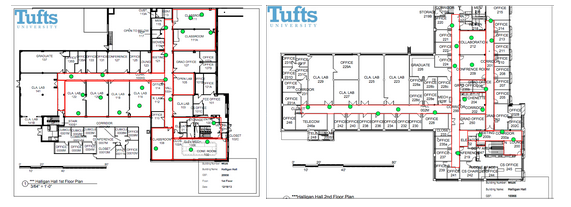
\includegraphics[width=\linewidth]{testpoints}
\begin{center}
Figure 3 - Test points on Halligan Floor 1 (left) and Floor 2 (right); red boxes indicate accessible regions, and green dots indicate test points
\end{center}

\indent These test points were used to evaluate our overall accuracy, which was broken into two sections: an examination of distance functions  and an examination of the map modifying techniques. The distance function comparison evaluates our modification to the Euclidean distance function and integration of the Jaccard distance, while the map modification section investigates the effect of neighbor-weighting and Jaccard floor detection.
	
\subsection{Distance Function Comparisons}
\indent We tested our WKNN algorithm iteratively using several values of K, and we found that the algorithm yields the greatest accuracy using K=3. Figure 4 shows the observed accuracy of our WKNN algorithm using four different distance functions: Euclidean distance (E), penalty-weighted Euclidean distance (E'), inverse Jaccard coefficient (J-1), and a linear combination of E' and J-1(E'+J-1). As the graph shows, the standard Euclidean distance metric performs significantly better than the inverse Jaccard coefficient, yielding an average error 4.73m as opposed to 7.33m. Modifying the Euclidean distance with an additional penalty factor results in another significant improvement, achieving an average error of 4.02m. Using a linear combination of the Euclidean distance and the inverse Jaccard coefficient only brings a slight performance increase, yielding an average error of 3.98m. 

\includegraphics[width=\linewidth]{CDFPos}
\begin{center}
Figure 4: CDF of positioning accuracy for various WKNN distance functions (K=3)
\end{center}

\subsection{Map Modification}
\indent Figure 5 shows the effect of introducing neighbor-weighting to our WKNN distance function. As expected, the neighbor-weighting addition does not appear to yield significant improvements for test points whose errors were relatively small. The WKNN algorithm located exactly 28 of 40 test points within 4m accuracy regardless of whether neighbor-weighting is used. However, using neighbor-weighting drops the maximum error from 22.49m to 7.74m, and it drops the average error from 3.98 m to 3.02m. For test points that were not located within 4m accuracy using the original distance function, introducing neighbor-weighting reduces the average error from 8.53m to 3.64m. \\

\includegraphics[width=\linewidth]{CDFNei}
\begin{center}
Figure 5: Effect of neighbor-weighting on localization accuracy (K=3)
\end{center}

\indent Figure 6 shows the effect of our floor detection pre-processing technique on runtime, assuming an average of 100 fingerprints per floor. In our current test environment which contains only two floors, no noticeable runtime improvement is seen when we determine the floor of a test point before running WKNN with a more complex distance metric. However, when we simulate an environment containing 100 floors over several buildings, our floor detection technique reduces localization time by 39.1$\%$, from 6.89 seconds to 4.20 seconds.

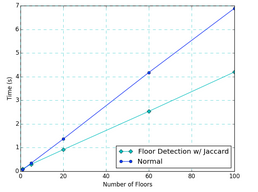
\includegraphics[width=\linewidth]{floorTime}
\begin{center}
Figure 6: Effect of floor detection pre-processing technique on localization time
\end{center}
	
%------------------------------------------------
\section{Discussion}

\indent Our positioning application has runtime and accuracy [10] similar to other fingerprint based systems. There are fingerprinting positioning systems with higher accuracy, many utilize application specific hardware whereas our application operates with no assumed site information, consumer hardware and less consistent data, making minimal requirements of the survey site. \\
\indent One specific example is the Microsoft RADAR system proposed in the 2000 IEEE paper which utilizes a basic KNN algorithm with RF signals. Although several systems have come out since RADAR that are improvements, the system achieved similar average error distances, 3 - 5 meters, while operating on a single floor which was highly arranged for the experiment, with the three base stations placed by the developing team, and a single set of hardware utilized. We believe that it is important to demonstrate that this level of accuracy can be realized currently with consumer hardware in a commercial-like setting. Similar to how RADAR was able to utilize techniques such as continual user tracking, and multiple radio maps for different environments such as time of day [12], we believe this implementation could be improved with these methods to reach even higher accuracy while still utilizing a device agnostic system. \\
\indent second system, proposed in 2013, uses improved double-peak Gaussian distributions and a probabilistic approach to determine position. This approach used a single device for mapping, and reports an average error of 1.5 meters [13]. While this is decidedly a higher accuracy, we believe that the techniques indicated in this paper and the RADAR improvements could be utilized to achieve a similar accuracy.
	
%------------------------------------------------

%\section{Results}

%\begin{table}[H]
%\caption{Example table}
%\centering
%\begin{tabular}{llr}
%\toprule
%\multicolumn{2}{c}{Name} \\
%\cmidrule(r){1-2}
%First name & Last Name & Grade \\
%\midrule
%John & Doe & $7.5$ \\
%Richard & Miles & $2$ \\
%\bottomrule
%\end{tabular}
%\end{table}

%\lipsum[5] % Dummy text

%\begin{equation}
%\label{eq:emc}
%e = mc^2
%\end{equation}

%\lipsum[6] % Dummy text



%----------------------------------------------------------------------------------------
%	REFERENCE LIST
%----------------------------------------------------------------------------------------

\begin{thebibliography}{99} % Bibliography - this is intentionally simple in this template

\bibitem{1} Sayed, Ali H., Alireza Tarighat, and Nima Khajehnouri.,
"Challenges Faced in Developing Techniques for Accurate Wireless Location Information."
\emph{IEEE Signal Processing Magazine. IEEE, 1}, July 2005. Web. 11 Mar. 2015.
 
\bibitem{2} Sayed, Ali H., Alireza Tarighat, and Nima Khajehnouri.,
"Performance Comparison of Indoor Positioning Techniques Based on Location Fingerprinting in Wireless Networks."
\emph{IEEE Xplore}, 1 Jan. 2005. Web. 11 Mar. 2015. 
 
\bibitem{3} Chaudhuri, K., D. Sanghi, and P. Bhagwat. ,
"Location Determination of a Mobile Device Using IEEE 802.11b Access Point Signals."
\emph{IEEE Xplore. IEEE}, 16 Mar. 2003. Web. 11 Mar. 2015.

\bibitem{4} Lakmali, B.D.S., and Dias, D. ,
"Database Correlation for GSM Location in Outdoor and Indoor Environments."
\emph{Information and Automation for Sustainability, 2008. ICIAFS 2008. 4th International Conference on, vol., no., pp.42,47,}, 12-14 Dec. 2008.
 
\bibitem{5} Kokkinis, Akis; Raspopoulos, Marios; Kanaris, Loizos; Liotta, Antonio; Stavrou, Stavros,
"Map-aided fingerprint-based indoor positioning,"
\emph{Personal Indoor and Mobile Radio Communications (PIMRC), 2013 IEEE 24th International Symposium on}, vol., no., pp.270,274, 8-11 Sept. 2013.

\bibitem{6} Dunbar, Daniel, and Greg Humphreys.,
"A Spatial Data Structure for Fast Poisson-Disk Sample Generation."
\emph{www.cs.virginia.edu. University of Virginia},  1 Jan. 2006. Web. 11 Mar. 2015. 

\bibitem{7} Machaj, Juraj, Peter Brida, and Robert Piche.,
?Rank Based Fingerprinting Algorithm for Indoor Positioning.?
\emph{ International Conference on Indoor Positioning and Indoor Navigation IPIN, Guimaraes, Portugal},  21-23 September 2011. Web. 12 Mar. 2015.

\bibitem{8} Fielding, R.,
"Architectural Styles and the Design of Network-based Software Architectures."
\emph{ (Unpublished Doctoral dissertation). University of California, Irvine.}, 200

\bibitem{9} Kemppi, P.; Nousiainen, S.
"Database Correlation Method for Multi-System Positioning,"
\emph{Vehicular Technology Conference, 2006. VTC 2006-Spring. IEEE 63rd },  vol.2, no., pp.866,870, 7-10 May 2006.

\bibitem{10} Hui Liu, Houshang Darabi, Pat Banerjee, and Jing Li.,
"Survey of Wireless Indoor Positioning Techniques and Systems,"
\emph{ (Systems, Man, and Cybernetics, Part C: Applications and Reviews, IEEE Transactions on.}, vol.37, no.6, pp.1067,1080, Nov. 2007 

\bibitem{11} P. Bahl and V. N. Padmanabhan,
?RADAR: An in-building RF-based user location and tracking system,?
\emph{in Proc. IEEE INFOCOM}, 2000, Mar., vol. 2, pp. 775?784.

\bibitem{12} P. Bahl and V. N. Padmanabhan,
?Enhancements to the RADAR user location and tracking system,?
\emph{Microsoft Corp., Tech. Rep. MSR-TR- 2000?12}, Feb. 2000.

\bibitem{13} Chen, Lina, Binghao Li, Kai Zhao, Chris Rizos, and Zhengqi Zheng,
"An Improved Algorithm to Generate a Wi-Fi Fingerprint Database for Indoor Positioning."
\emph{Sensors (Basel, Switzerland). Molecular Diversity Preservation International (MDPI)}, 8 Aug. 2013. Web. 03 Apr. 2015.


\end{thebibliography}
%----------------------------------------------------------------------------------------

\end{multicols}

\end{document}

